% ****** Start of file apssamp.tex ******
%
%   This file is part of the APS files in the REVTeX 4.1 distribution.
%   Version 4.1r of REVTeX, August 2010
%
%   Copyright (c) 2009, 2010 The American Physical Society.
%
%   See the REVTeX 4 README file for restrictions and more information.
%
% TeX'ing this file requires that you have AMS-LaTeX 2.0 installed
% as well as the rest of the prerequisites for REVTeX 4.1
%
% See the REVTeX 4 README file
% It also requires running BibTeX. The commands are as follows:
%
%  1)  latex apssamp.tex
%  2)  bibtex apssamp
%  3)  latex apssamp.tex
%  4)  latex apssamp.tex
%
\documentclass[%
%superscriptaddress,
%groupedaddress,
%unsortedaddress,
%runinaddress,
%frontmatterverbose, 
%preprint,
%showpacs,preprintnumbers,
%nofootinbib,
%nobibnotes,
%bibnotes,
 amsmath,amssymb,
 aps,
 twocolumn,
 prl,
 reprint,
%pra,
%prb,
%rmp,
%prstab,
%prstper,
floatfix,
]{revtex4-1}

\usepackage{graphicx}% Include figure files
\usepackage{dcolumn}% Align table columns on decimal point
\usepackage{bm}% bold math
\usepackage{lineno}
%\addbibresource{references.bib}
\linenumbers % Commence numbering lines
%\usepackage{hyperref}% add hypertext capabilities
%\usepackage[mathlines]{lineno}% Enable numbering of text and display math
%\linenumbers\relax % Commence numbering lines

%\usepackage[showframe,%Uncomment any one of the following lines to test 
%%scale=0.7, marginratio={1:1, 2:3}, ignoreall,% default settings
%%text={7in,10in},centering,
%%margin=1.5in,
%%total={6.5in,8.75in}, top=1.2in, left=0.9in, includefoot,
%%height=10in,a5paper,hmargin={3cm,0.8in},
%]{geometry}

\begin{document}

\preprint{APS/123-QED}

\title{Matching Matched Filtering with Deep Networks in Gravitational wave Astronomy}

\author{Hunter Gabbard}
 \email{Corresponding author: h.gabbard.1@research.gla.ac.uk}
\author{Fergus Hayes}
\author{Chris Messenger}
\author{Michael Williams}
\affiliation{
 SUPA, School of Physics and Astronomy, \\
 University of Glasgow, \\
 Glasgow G12 8QQ, United Kingdom \\
}

\date{\today}% It is always \today, today,
             %  but any date may be explicitly specified

\begin{abstract}
 We report a new method for classifying gravitational-wave (GW) signals from binary black hole (BBH) mergers using a deep convolutional neural network. Using only the raw time series as an input, we are able to distinguish GW signals injected in Gaussian noise amongst instances of purely Gaussian noise time series with (\textbf{need figure of merit here}) percent accuracy. We compare our results with the standard method of matched filtering used in Advanced LIGO and find the methods to be comparable.  
\begin{description}
\item[PACS numbers]
May be entered using the \verb+\pacs{#1}+ command.
\end{description}
\end{abstract}

\pacs{Valid PACS appear here}% PACS, the Physics and Astronomy
                             % Classification Scheme.
%\keywords{Suggested keywords}%Use showkeys class option if keyword
                              %display desired
\maketitle

%\tableofcontents


\textit{Introduction} --- The field of gravitational wave astronomy has seen an explosion of binary black hole detections over the past several years \cite{PhysRevLett.116.061102, PhysRevLett.116.241103, PhysRevLett.118.221101}. These detections were made possible by the Advanced Laser Interferometer Gravitational wave Observatory (aLIGO) detectors, as well as the recent joint detection of GW170814 with Advanced Virgo \cite{PhysRevLett.119.141101}. Over the coming years many more such observations, including other more exotic sources such as binary neutron star (BNS), intermediate black hole (IMBH), and neutron star black hole (NSBH) mergers, are likely to be observed on a more frequent basis. As such, the need for more efficient search methods will be more pertinent as the detectors increase in \textit{volume} $\times$ \textit{time} sensitivity.

The algorithms used to make these detections \cite{0264-9381-33-21-215004} [\textbf{cite gstlal too??}] are computationally expensive to run. Part of the reason being that the methods used by these \textit{search pipelines} are complex, sophisticated processes run over a large parameter space using advanced signal processing techniques. Distinguishing noise from signal in this search pipeline, and others like it, is done using a technique called matched template filtering. Matched template filtering uses a \textit{bank} of template waveforms that spans the astrophysical parameter space \cite{PhysRevD.44.3819, PhysRevD.49.1707, PhysRevD.53.6749, PhysRevD.60.022002, 0264-9381-23-18-002, PhysRevD.80.104014, PhysRevD.86.084017, PhysRevD.89.084041, PhysRevD.87.124003, 1307.4158, PhysRevD.89.024003, PhysRevD.93.124007}. We span a large astrophysical parameters space because we do not know \textit{a priori} what the parameters of the gravitational waves in the data are. Because the waveforms of the signals are well modeled, the pipeline uses matched filtering to search for those signals burried in the detector noise. More on how we implement this technique in comparisons with our model will be mentioned later in the methods section of this letter.

We propose that a deep learning algorithm which requires only the raw data time series as input with minimum signal processing would be one alternative search method. This pipeline would be able to be pretrained and then run on real-time detector data with maximum efficiency, as well as in low-latency.

Deep learning is a subset of machine learning which has gained in popularity over the past several years \cite{NIPS2012_4824, 1406.2661, 1409.1556, 1412.7062, 1311.2901, 1409.4842}. A deep learning algorithm is composed of arrays of processing units, called neurons, which can be anywhere from one to several layers deep (\textbf{explain more about what a neuron is?}). Deep learning algorithms typically consist of an input layer, followed by one to several hidden layers and then one to $N$ neurons that output a single value each. This value can then either be used to solve classfication, or regression-like problems. In the case of classification, each output neuron corresponds to the probability that a particular sample is of a certain class. 

In our model, we use a variant of a deep learning algorithm called a convolutional neural network (CNN) \cite{726791}. CNN layers are composed of five primary variants: input, convolutional, activation, pooling, and fully-connected. Where input holds the raw pixel values of the sample image, the convolutional layer computes the convolution between the kernel and a local region of the input layer volume, activation applies an elementwise activation function leaving the size of the previous layer's output volume unchanged, pooling performs a downsampling operation along the spatial dimensions, and the fully-connected layer computes the class scores using an error function, cross-entropy, defined as

\begin{equation} \label{eq:loss}
f_{\theta^{'}}(\theta) = -\sum_{i} \theta_{i}^{'} \mathrm{log}(\theta_{i}),
\end{equation}

where $\theta_{i}$ is the predicted probability distribution of class $i$ and $\theta_{i}$ is the true probability for that class \cite{tensorflow2015-whitepaper}. 

In the following sections we will discuss our choice of network architecture and tuning of it's hyperparameters, compare the results of our network with the widely used GW signal classification technique called matched filtering, and comment on future improvements related to this work.      

\textit{Methods} --- In this analysis, in order to make the problem simple, we only distinguish between BBH merger signals injected into a Gaussian noise time series from pure white Gaussian noise time series. The time series for both classes of signals are 1s in duration sampled at 8192 Hz. \textbf{say more about how noise and injection are generated using Chris's code.} 

For our noise signals we generate a power spectrum density (PSD) that is comparable to aLIGO design sensitivity using a library of gravitational wave data analysis routines called \texttt{LALSuite}. That PSD is then converted to an amplitude time series where a random phase shift is given to each spectral component. The inverse real fast fourier transform (IFFT) is then applied and returns a Gaussian time series.

Injections are made using the IMRPhenomD type waveform \cite{PhysRevD.93.044006, PhysRevD.93.044007} where the component masses of the waveform range from 5\(M_\odot\) to 100\(M_\odot\), $m_{1} > m_{2}$, and all with zero spin (\textbf{not sure if correct?}). Each injection is given a random sky location. The waveforms are then randomly placed within the time series, see figure \ref{fig:waveform}, where the peak of the waveform is within the last $20$\% of the time series (\textbf{perhaps give reason for why this is done}). The waveform is normalised using the integrated signal-to-noise ratio (iSNR), where SNR is defined as

\begin{equation} \label{eq:snr}
\rho_{opt}^{2} = 4 \int_{0}^{\inf} \frac{\lvert \hat{h(f)}\rvert^{2}}{S_{n}(f)} \mathrm{d}f,
\end{equation}

where $\rho_{opt}$ is the optimal SNR, $\hat{h(f)}$ is the strain amplitude, and $S_{n}(f)$ is the PSD.

In our runs we used $1,000$ Gaussian noise signals and $1,000$ unique injections with over $25$ varrying noise realizations resulting in a total of $50,000$ samples. The samples are then arranged in the form of a $1 \times 8192$ pixel sample which is scaled by the GW strain amplitude, $h(t)$, over one color channel (grayscale). (\textbf{give ligo definition of optimal SNR}) $70\%$ of these samples are used for training, $15\%$ for validation, and $15\%$ for testing. 

\begin{figure}
 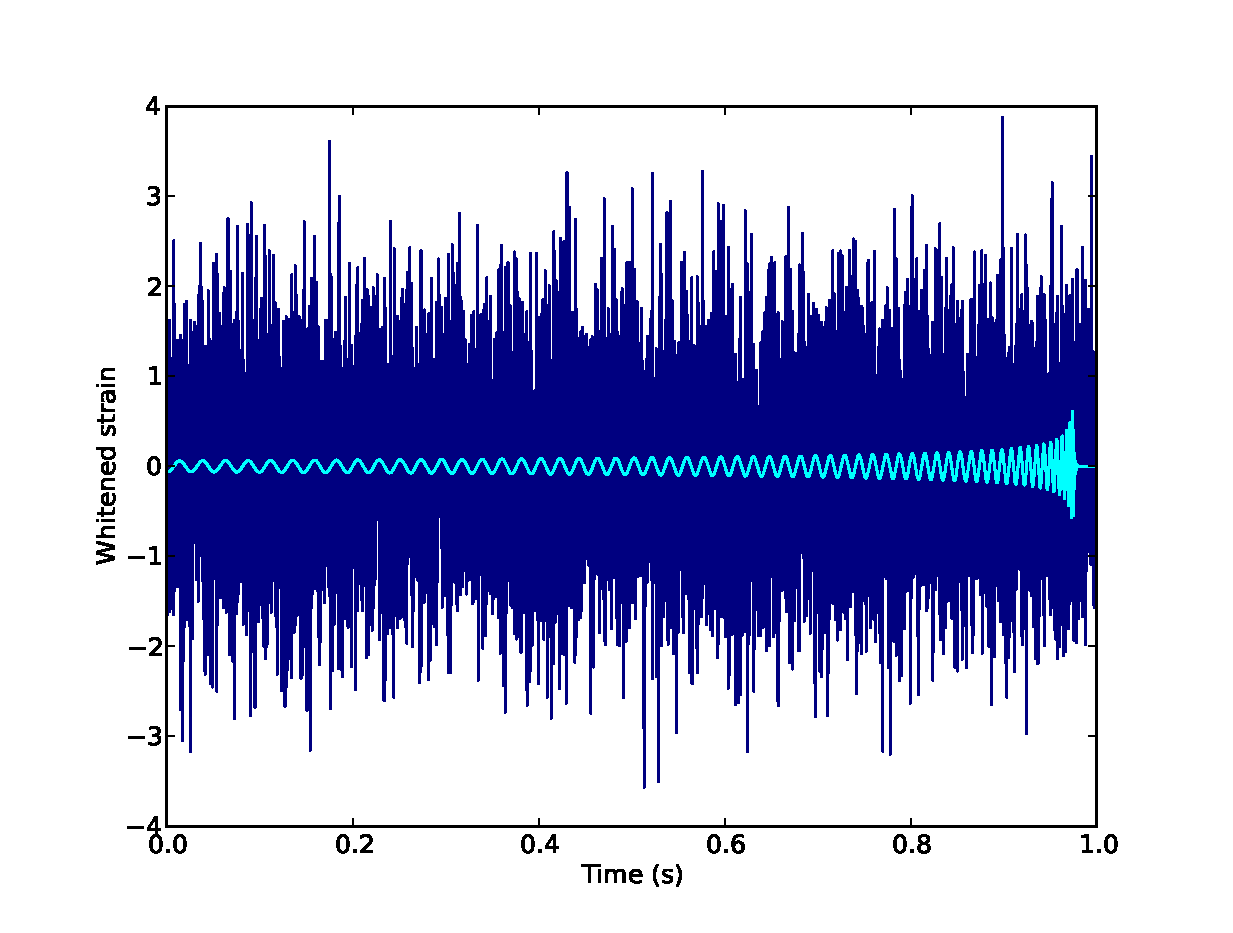
\includegraphics[width=0.5\textwidth]
 {figures/waveform.eps}
 \caption{\label{fig:waveform} Description here.}
\end{figure}

In order to achieve the optimal network, multiple sets of hyperparameters are tuned. First, we rescaled the data, but with the existing setup, this did not seem to improve upon the performance. We also attempted applying transfer learning where we used networks trained on successively higher SNR values, though performance benefits were minimal. Network depth was adjusted between 2 to 10 convolutional layers. Our initial data set needed at least 4 convolutional layers. Later data sets with various noise realizations needed fewer convolutional layers to perform comparatively well, but adding more layers still seemed to improved performance. The inclusion of dropout was used within the fully-connected layers as a form of regularization.

For updating our weights and bias parameters (in order to minimize our loss function, $f(\theta)$, \eqref{eq:loss}) we settled on the nesterov momentum optimization function

\begin{equation} \label{eq:nesterov1}
v_{t+1} = \mu v_{t} - \epsilon \nabla f(\theta_{t} + \mu v_{t}),
\end{equation}

\begin{equation} \label{eq:nesterov2}
\theta_{t+1} = \theta_{t} + v_{t+1},
\end{equation} \\

where $\epsilon > 0$ is the learning rate, $\mu \in [0,1]$ is the momentum coefficient, and $\nabla f(\theta_{t})$ is the gradient with respect to the weight vector $\theta_{t}$. Nesterov momentum was the ideal choice because of its prescient ability to approximate the next position of the weights and bias parameters which therefore gives a rough approximation of their values (\textbf{perhaps this is a bit off topic}). Thus the gradient is calculated not with respect to the current parameters, but with respect to the approximate future positions of those parameters \cite{Sutskever:2013:IIM:3042817.3043064}. A further detailed description of the neural network architecture used can be found in Table \ref{table:network}.

\begin{figure}[!h]
 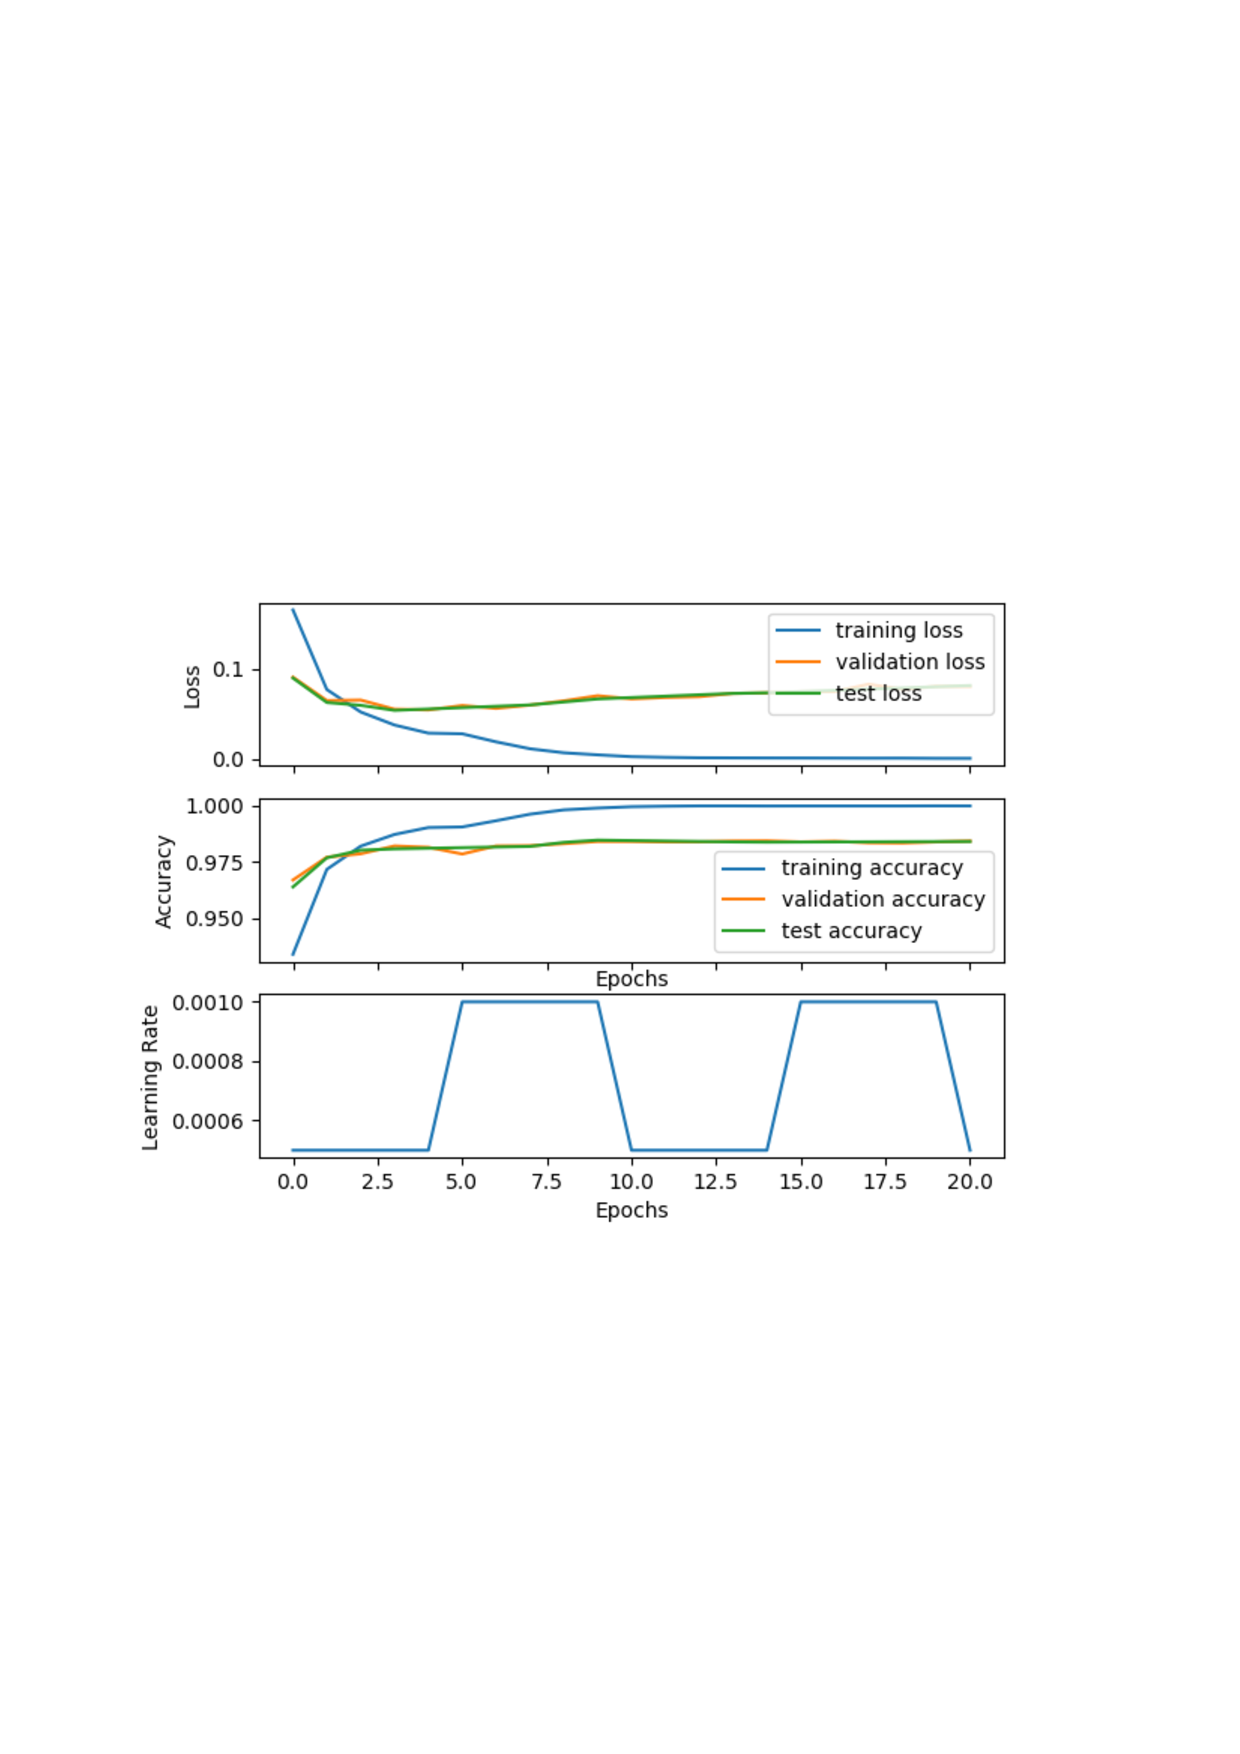
\includegraphics[width=0.5\textwidth]
 {figures/loss.png}
 \caption{\label{fig:loss_curve} The loss, accuracy and learning rate plots (shown above) illustrate how the network's performance is defined as a function of the number of training epochs. The goal is to minimize the loss function, which will in turn maximize the accuracy of the classifier. The first initial epochs see an exponential decrease in the loss function and then a slowly falling monotonic curve to follow. This indicates that the longer our network is trained, a limit with respect to the accuracy is approached. In our case, we cyclically adjust the learning rate to oscialte between $5 \times 10^{-4}$ and $1 \times 10^{-3}$ at a constant frequency. Studies have shown that this policy of learning rate adjustement (\textbf{should replace figure with better run})
}
\end{figure}

Largely following matched filtering techniques used on the LIGO Open Science Center optimal matched filter page \cite{1742-6596-610-1-012021} we compare our results to the standard optimal matched filtering process used by aLIGO \cite{PhysRevD.85.122006}. Considering the example of one candidate GW signal, we iterate over a comprehensive template bank. The template bank was generated using 8000 randomly sampled mass pairs from the same distribution with no adjustment to assure the parameter space was adequately covered. For each template, we compute the Fast Fourier Transform (FFT) of the data and the template, where the template has been zero padded in order for both to be of the same length. Finally, we multiply the fft'd template and data together and divide by the PSD. An inverse FFT is then applied in order to convert back to the time domain. The output is then normalized so that we have an expected value of 1 for pure Gaussian noise.

\begin{table*}[]
\centering
\caption{The optimal network structure (seen below) was determined through multiple tests and tunnings of hyperparameters by means of trial and error. The network consists of 8 convolutional layers, followed by 2 fully-connected layers. Max-pooling is performed on the first, fifth, and eigth layer, whereas dropout is only performed on the two fully-connected layers. Each layer uses an Elu activation function while the last layer uses a Softmax activation function in order to normalize the output values to be between zero and one so as to give a probability value for each class. \\} 
\label{table:network}
\begin{tabular}{lllllllllll}
                    & layer 1 & layer 2 & layer 3 & layer 4 & layer 5 & layer 6 & layer 7 & layer 8 & layer 9 & layer 10 \\
Number of Kernals   & 8       & 16      & 16      & 32      & 64      & 64      & 128     & 128     & 64      & 2        \\
Filter Size         & 32      & 16      & 16      & 16      & 8       & 8       & 4       & 4       & n/a     & n/a      \\
Max Pooling         & yes       & no       & no       & no       & yes       & no       & no       & yes       & no     & no      \\
Fully Connected     & no     & no     & no     & no     & no     & no     & no     & no     & yes     & yes      \\
Drop out            & 0.0     & 0.0     & 0.0     & 0.0     & 0.0     & 0.0     & 0.0     & 0.0     & 0.5     & 0.5      \\
Activation Function & Elu     & Elu     & Elu     & Elu     & Elu     & Elu     & Elu     & Elu     & Elu     & Softmax 
\end{tabular}
\end{table*}

\textit{Results} --- After tunning several hyperparameters and then settling on an ideal network format (Table \ref{table:network}), we present the results of our classifier on a noise vs. injection sample set. We trained our network using a transfer learning approach whereby we initially trained our network on a sample set of 1000 noise and 1000 injection signals (each with 25 different noise realizations) with an integrated SNR value of 12. We then lowered the integrated SNR value by 2 and (using the same weights from our previous network) we trained our classifier again. This approach seemed to only have a marginal benefit on the overall performance of the classifier.  

The confusion matrix in figure \ref{fig:confusion} shows $99.86\%$ accuracy with triggers at an integrated SNR of 12, $99.64\%$ accuracy with integrated SNR 10, $97.88\%$ at integrated SNR 8, $88.72\%$ at an integrated SNR of 6, $68.34\%$ at integrated SNR 4, and $50.19\%$ accuracy at integrated SNR 2.


\begin{figure}[]
 
 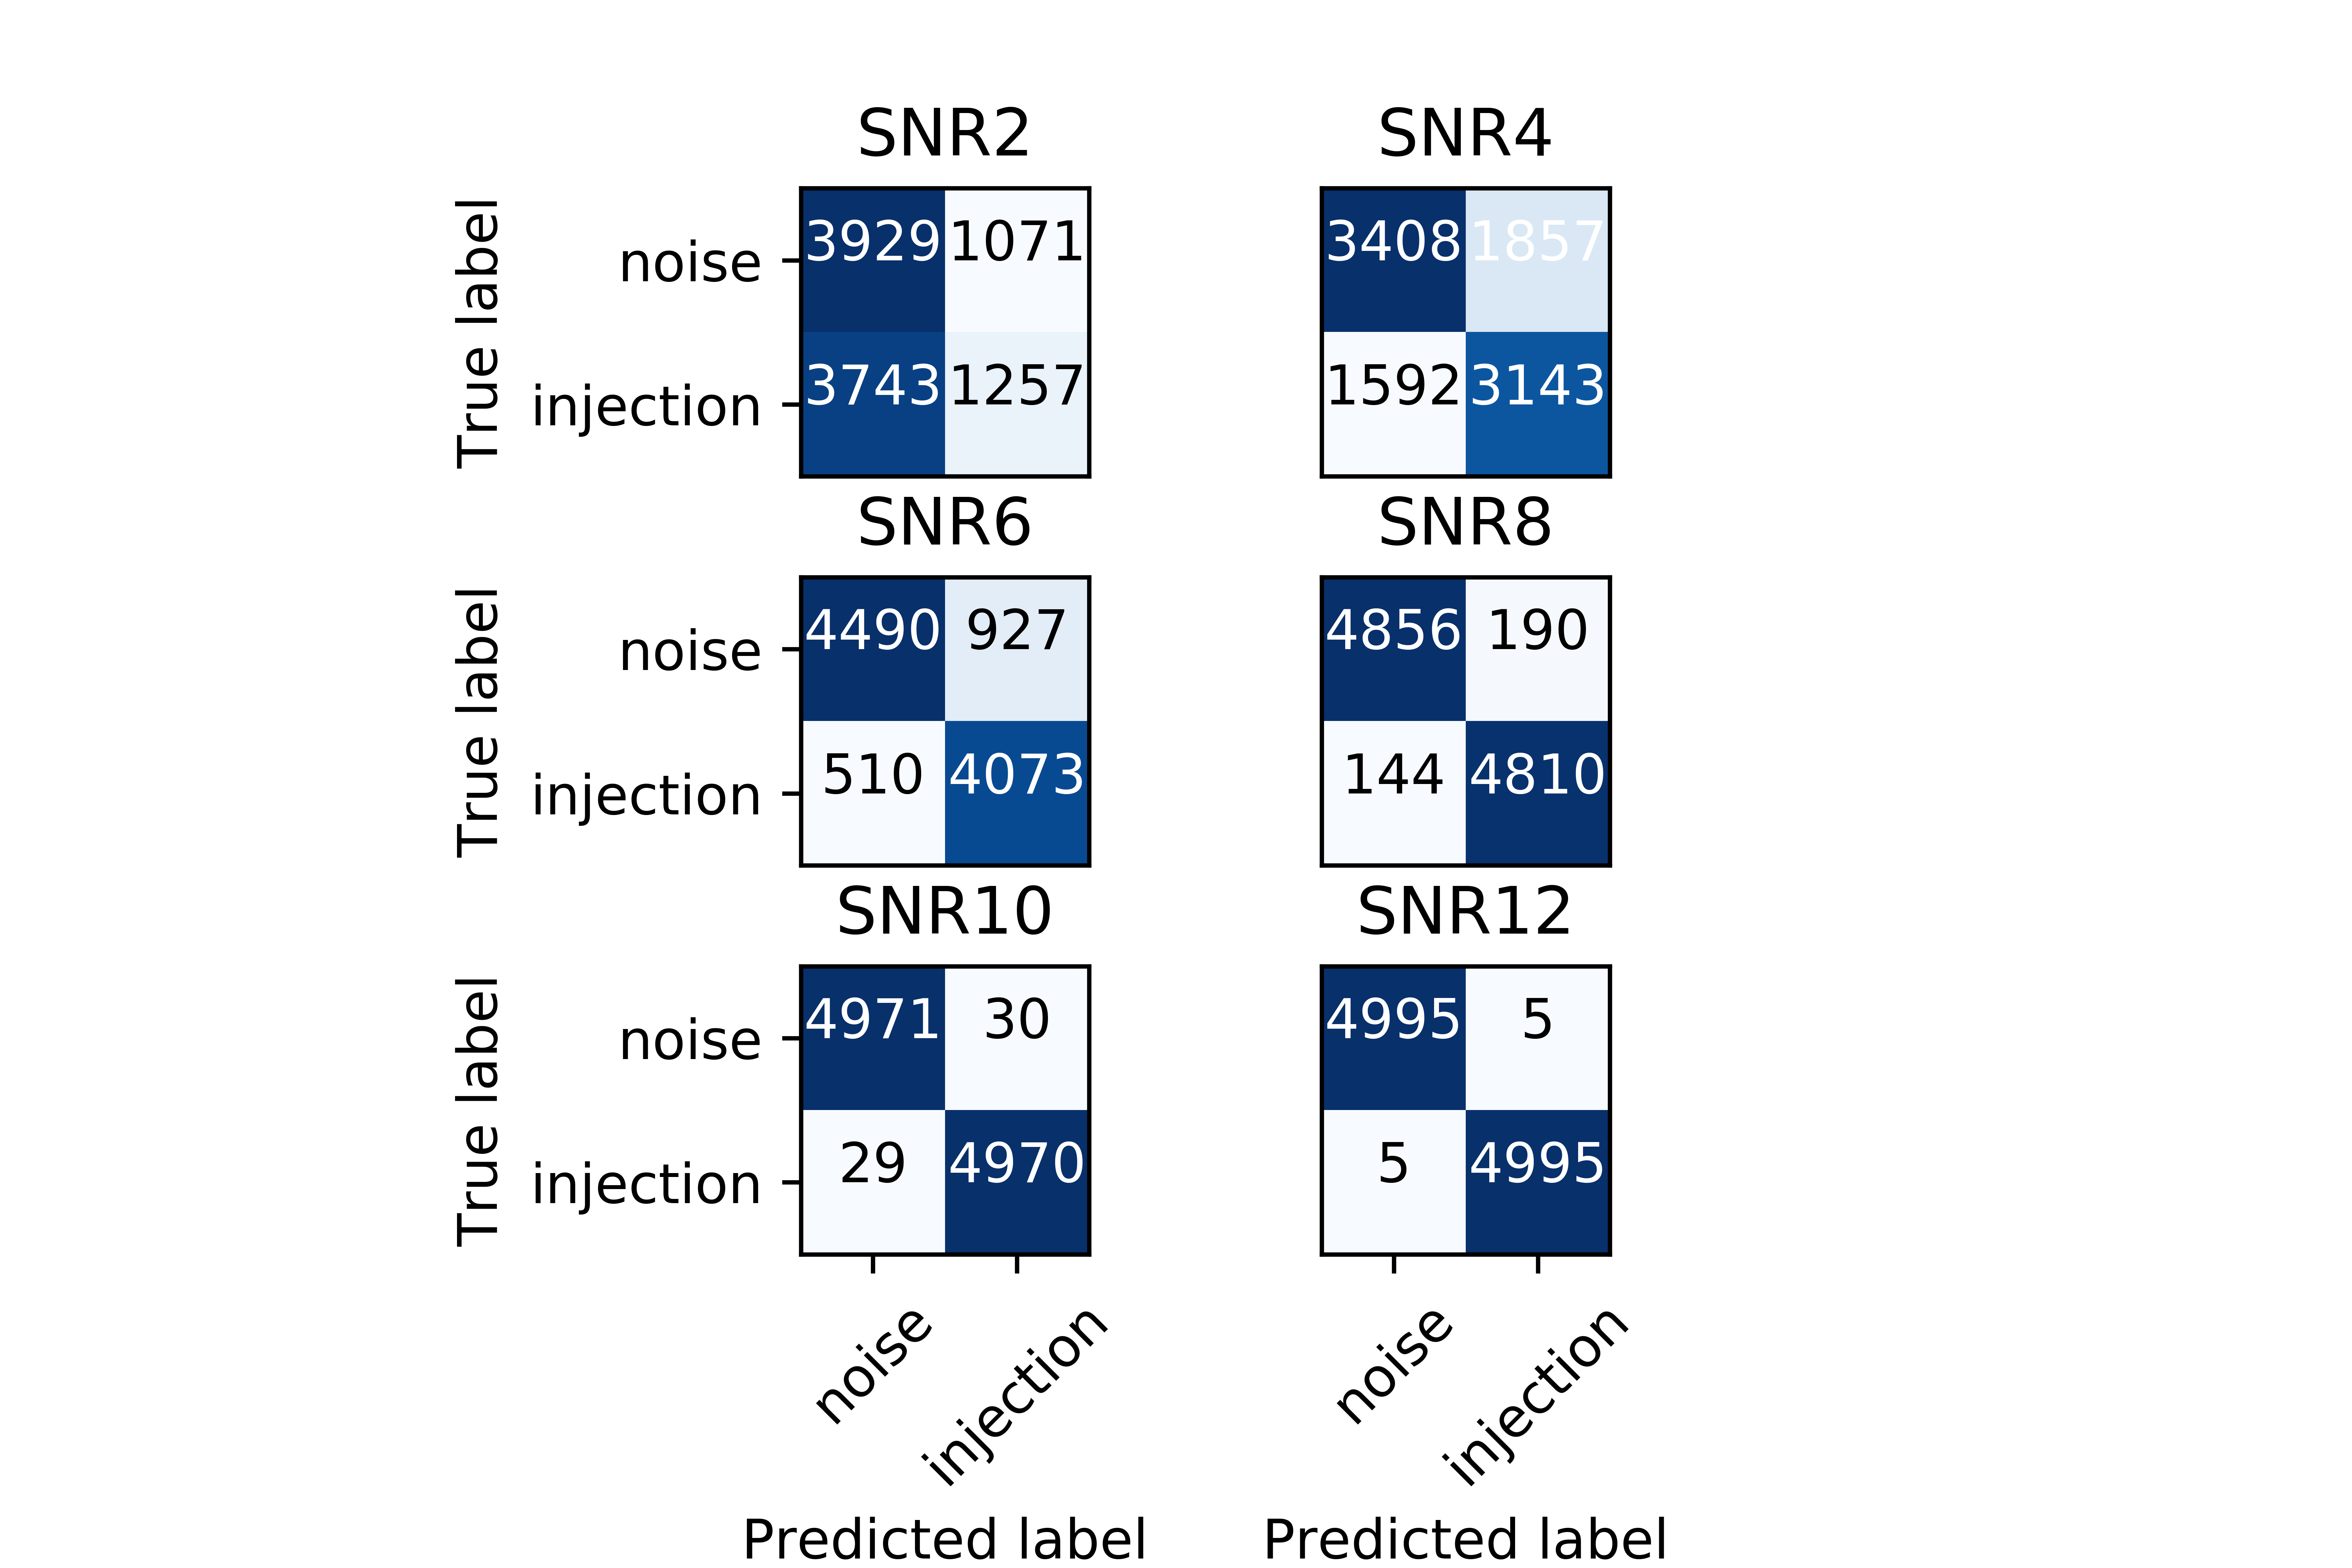
\includegraphics[width=0.5\textwidth]
 {figures/confusion_matrix.eps}
 \caption{\label{fig:confusion} Confusion matrices for runs from iSNR 2 - iSNR 12. The accuracies for all are listed as follows: $50.19\%$ at iSNR 2, $68.34\%$ at iSNR 4, $88.72\%$ at iSNR 6, $97.88\%$ at iSNR 8, $99.64\%$ at iSNR 10 and $99.86\%$ at iSNR 12. Note that runs with iSNR 2 give results that are equivalent randomized guessing.}
\end{figure}

In figure \ref{fig:ROC_curve} we compare our results to that of matched filtering where we use two alternative match filtering methods. The first, using the nominal template bank described in the \textit{Methods} section, whereas the second uses the optimal template for each injection, whereby optimal is defined as the template used to generate that injection. As seen in figure \ref{fig:ROC_curve} all three methods have equivalent performance proficiency at $\sim \mathrm{iSNR} > 9$, whereas there is a marginal dip in performance in the nominal matched filtering method and our deep learning classifier. It should be noted that our classifier exceeds the performance proficiency of that of the nominal matched filtering method between iSNR 2 and iSNR 4. 

\begin{figure}[]
 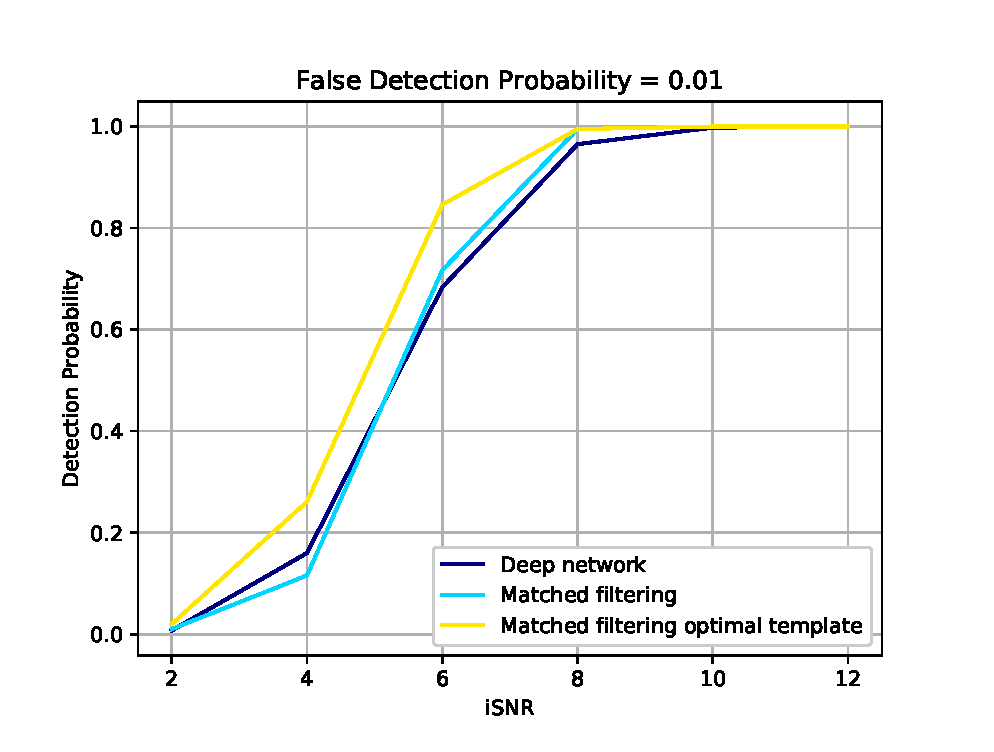
\includegraphics[width=0.5\textwidth]
 {figures/accuracy.eps}
 \caption{\label{fig:ROC_curve} \textbf{Place description here.}}
\end{figure}

We compare the results of all three methods at various injection iSNR values in figure \ref{fig:isnr_curves}. It is not surprising to see that the matched filtering method using the optimal template consistantly performs better than both the nominal match filtering method and our deep learning classifier. However, what is considerable is the comparison between the nominal matched filtering and the deep learning classifier detection probability curves. It can clearly be seen that our classifier exceeds the performance of the nominal matched filtering method at iSNR 2, 4 and 6. This is a promising result and certainly merits further investigation.  

\begin{figure}[]
 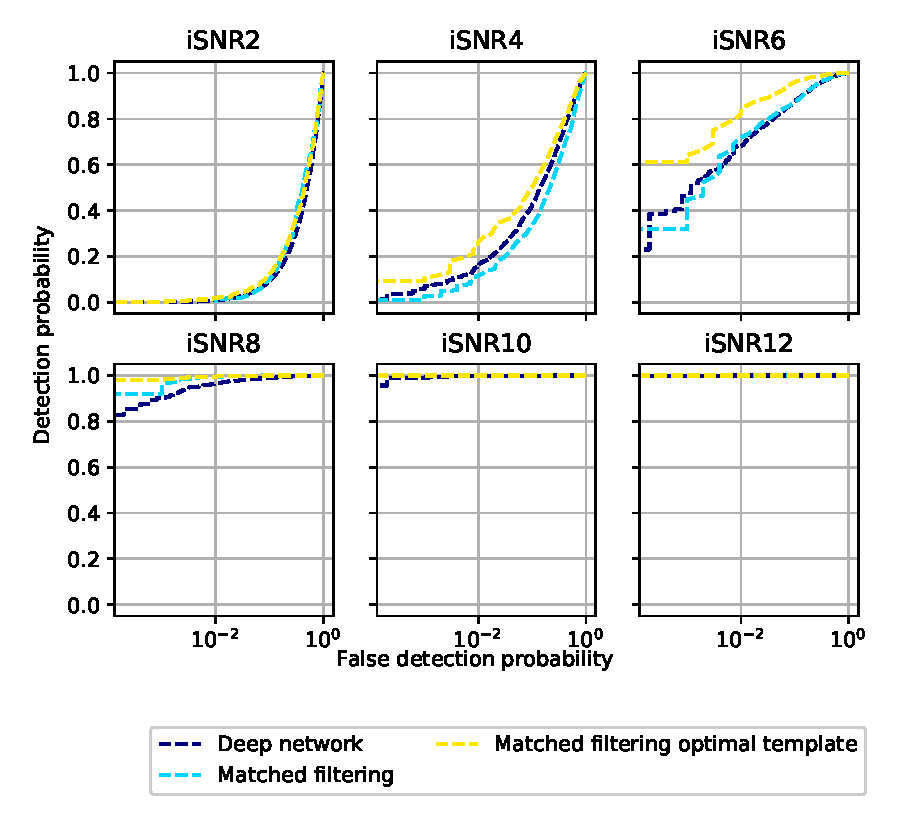
\includegraphics[width=0.5\textwidth]
 {figures/ROC_curves.eps}
 \caption{\label{fig:isnr_curves} \textbf{Place description here.}}
\end{figure}

\textit{Conclusions} --- In conclusion, we demonstrate that deep learning, when applied to a raw data time series, is able to produce equivalent results to matched template filtering. We employ a deep convolutional neural network with carefully chosen hyperparamters and produce an output that returns the class probability value of any given signal. This output could then further be applied as a ranking statistic in the aLIGO CBC search. Although only BBH mergers were used, this method could also easily be applied to other merger types, such as BNS and NSBH signals. The results shown in both figure \ref{fig:ROC_curve} and figure \ref{fig:isnr_curves} indicate that deep learning approaches even have the unprecedented potential to entirely exceed matched template filtering. 

This work was supported by blah blah blah, something something, important people ... 



% The \nocite command causes all entries in a bibliography to be printed out
% whether or not they are actually referenced in the text. This is appropriate
% for the sample file to show the different styles of references, but authors
% most likely will not want to use it.

\bibliographystyle{apsrev4-1}
\bibliography{references}% Produces the bibliography via BibTeX.


\end{document}
%
% ****** End of file apssamp.tex ******
